\section{Frontend alkalmazás}

A felhasználó egy webes felületet lát az alkalmazásból (a design munkákat
ezúton is köszönöm Sári Tamásnak),
a feladata, hogy egy egyszerű SPA-t (Single Page Application) biztosítson,
illetve a különböző interakciókat a megfelelő alrendszereknek továbbítsa.

A frontend szerver egy Nginx \emph{reverse proxy} mögött foglal helyet,
ami a statikus fájlokat (lefordított \verb=stylus= stílusfájlok, illetve
\verb=browserify= bundle-ök, képek) szolgál ki, minden egyéb kérést
a koa szervernek továbbít.

Alapesetben a felhasználó egy statikus HTML oldalra érkezik,
ami csak azért felelős, hogy a CSS stílusfájlok, illetve a kliensoldali JS
állományok betöltődjenek. Ezek után a felhasználó csak AJAX kéréseken keresztül
kommunikál a szerverrel.

A szerver feladata, hogy elindítsa az OAuth autentikációt, a végén keletkező
tokent az adatbázisban eltárolja, valamint beütemezze a megfelelő jobokat,
illetve ha ha ezek befejeződtek, akkor az elkészült statisztikákat
a kliensoldali alkalmazásnak eljuttassa.

\begin{figure}[h!]
  \centering
  
\includegraphics[width=0.5\textwidth]{figures/frontend-1}
  \caption{Az alkalmazás kezdő képernyője}
  \label{fig:frontend-1}
\end{figure}

\begin{figure}[h!]
  \centering
  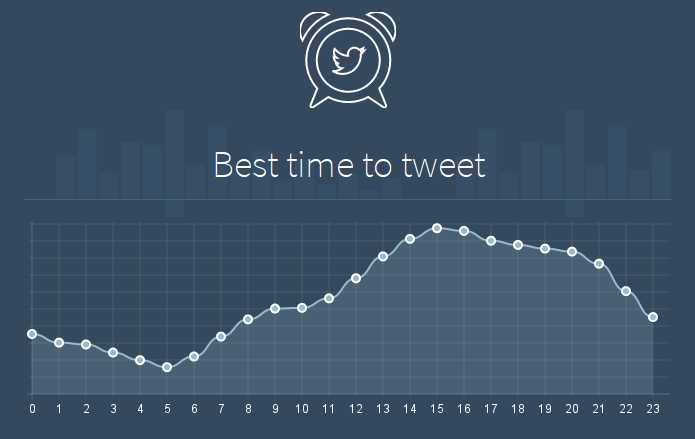
\includegraphics[width=0.5\textwidth]{figures/frontend-2}
  \caption{Az elkészült statisztika grafikonja}
  \label{fig:frontend-1}
\end{figure}
